\documentclass[12pt,a4paper,oneside,openany]{article}
\usepackage[utf8]{inputenc}
\usepackage{float}
\usepackage{array}
\usepackage{tabularx}
\usepackage{amsmath}
\usepackage[brazil]{babel}
\usepackage{breakurl}
\usepackage{graphicx}
\usepackage{geometry}
\geometry{a4paper,left=3cm,right=2cm,top=3cm,bottom=2cm}
\usepackage{hyperref}
\hypersetup{breaklinks=true}
\usepackage[backend=bibtex,style=authoryear,natbib]{biblatex}
\addbibresource{bibliografia.bib} % Arquivo com as referências bibliográficas





\geometry{a4paper, margin=1in}

\title{Comparação entre SVM e Redes Neurais MLP na Classificação de Tumores de Câncer de Mama}
\author{Alexandre Pereira Santos\\
Faculdade de Tecnologia SENAI de Desenvolvimento Gerencial\\
Pós-graduação Lato Sensu - MBA em Big Data e Machine Learning}
\date{December 17, 2024}

\begin{document}

\maketitle

\section*{Resumo}
O câncer de mama é o tipo mais prevalente entre mulheres em todo o mundo, representando cerca de 25\% dos casos globais. Este estudo investiga a aplicação de algoritmos de aprendizado de máquina para classificar tumores como malignos ou benignos. Foram utilizados os algoritmos Support Vector Machines (SVM) e Redes Neurais MultiLayer Perceptron (MLP) no conjunto de dados Wisconsin (diagnóstico). A metodologia incluiu pré-processamento, validação cruzada e otimização de hiperparâmetros para maximizar o desempenho dos modelos. Os resultados indicam que ambas as abordagens são promissoras no suporte ao diagnóstico precoce, com implicações significativas para a saúde pública. Esses achados reforçam o potencial do aprendizado de máquina como ferramenta auxiliar no diagnóstico clínico de câncer de mama, destacando sua relevância para a saúde pública. Os resultados demonstram que o SVM com kernel RBF obteve uma acurácia de 97,2\%, enquanto o MLP alcançou 98,1\% após otimizações.

\noindent \textbf{Palavras-chave:} Câncer de mama, aprendizado de máquina, classificação de tumores, Support Vector Machines (SVM), Redes Neurais MultiLayer Perceptron (MLP), diagnóstico precoce, saúde pública.

\section*{Abstract}
Breast cancer is the most prevalent type of cancer among women worldwide, accounting for approximately 25\% of global cases. This study investigates the application of machine learning algorithms to classify tumors as malignant or benign. Support Vector Machines (SVMs) and MultiLayer Perceptron (MLP) Neural Networks were employed on the Wisconsin Diagnostic Dataset. The methodology included preprocessing, cross-validation, and hyperparameter optimization to maximize model performance. The results indicate that both approaches are promising in supporting early diagnosis, with significant implications for public health. The results demonstrate that the SVM with the RBF kernel achieved an accuracy of 97.2\%, while the MLP reached 98.1\% after optimizations.

\noindent\textbf{Keywords:} Breast cancer, machine learning, tumor classification, Support Vector Machines (SVM), MultiLayer Perceptron Neural Networks (MLP), early diagnosis, public health.


\section{Introdução}

O câncer é uma das principais causas de morbimortalidade no mundo, com impactos significativos na saúde pública e na qualidade de vida dos pacientes. Segundo o Ministério da Saúde, o câncer, ou tumor maligno, refere-se a um grupo de mais de 100 doenças que compartilham o crescimento desordenado de células, capazes de invadir tecidos adjacentes e disseminar-se para outros órgãos por meio de metástases. A origem do câncer está diretamente associada a mutações no DNA celular, que alteram as instruções genéticas responsáveis por regular o ciclo de vida das células. Essas alterações podem levar ao surgimento de células anormais, cujo comportamento descontrolado resulta na formação de tumores malignos (Ministério da Saúde, 2024).

\noindent O câncer de mama destaca-se pela elevada prevalência e pelo impacto significativo na mortalidade feminina. De acordo com o Instituto Nacional do Câncer (INCA), é o segundo tipo mais frequente entre as mulheres, superado apenas pelo câncer de pele não melanoma. Globalmente, representa cerca de 25\% dos casos de câncer em mulheres, consolidando-se como uma das principais ameaças à saúde feminina. Embora raro antes dos 35 anos, sua incidência aumenta progressivamente com a idade. Uma notícia alentadora é que a detecção precoce e o tratamento adequado podem elevar as taxas de cura para até 95\% (Mulher Consciente, 2024).

\noindent A complexidade biológica do câncer de mama reflete a interação de fatores genéticos, hormonais, ambientais e comportamentais, tornando seu diagnóstico e manejo clínicos desafiadores. Um dos principais entraves é a distinção precisa entre tumores benignos e malignos, especialmente nas fases iniciais da doença. Métodos tradicionais, como mamografia e análise histopatológica, embora eficazes, podem ser limitados em sensibilidade ou especificidade, exigindo abordagens complementares para aumentar a confiabilidade diagnóstica.

\noindent A aplicação de algoritmos de aprendizado de máquina, como Support Vector Machines (SVM) e Multi-Layer Perceptrons (MLP), na medicina. O SVM é eficaz para tarefas de classificação, como diagnóstico de doenças, separando dados de diferentes categorias, como em exames de imagem para detecção de câncer. O MLP, utilizado na análise de imagens médicas, é capaz de reconhecer padrões complexos e pode ser empregado para prever resultados de tratamentos. Ambos os algoritmos auxiliam na melhoria do diagnóstico e prognóstico médico, otimizando tratamentos (Fonte: PAIXÃO, 2023).

\noindent Nesse contexto, o avanço das tecnologias de aprendizado de máquina (AM) tem se mostrado revolucionário. Ferramentas como Support Vector Machines (SVMs) e Redes Neurais MultiLayer Perceptron (MLPs) oferecem uma nova dimensão na análise de dados médicos. Com a capacidade de processar grandes volumes de informações e identificar padrões complexos, esses algoritmos têm o potencial de transformar a prática clínica, auxiliando na detecção precoce e na classificação de tumores de forma mais precisa e eficiente.

\noindent O conjunto de dados Wisconsin (Wolberg et al., 1995) é amplamente reconhecido na literatura científica como uma base de referência para estudos de aprendizado de máquinas voltados ao diagnóstico de câncer de mama. Com 30 atributos detalhados, incluindo características como textura, perímetro e simetria das células, este dataset oferece uma plataforma robusta para a construção e validação de modelos preditivos.

\noindent Este estudo investiga o desempenho de algoritmos de aprendizado de máquina, especificamente SVMs e MLPs, na classificação de tumores de mama como malignos ou benignos, utilizando o dataset Wisconsin. A abordagem metodológica incluiu pré-processamento dos dados, validação cruzada e otimização de hiperparâmetros para maximizar a acurácia e outras métricas de desempenho. Os resultados obtidos não apenas demonstram a eficácia dessas técnicas no suporte ao diagnóstico clínico, mas também destacam suas potenciais implicações para a saúde pública, especialmente em contextos de alta demanda e recursos limitados.

\noindent Combinando rigor técnico e aplicabilidade prática, este estudo reforça o papel central do aprendizado de máquina como ferramenta transformadora na luta contra o câncer de mama. Além disso, busca ampliar a compreensão sobre os desafios e oportunidades no uso dessas tecnologias, promovendo sua integração cada vez mais efetiva nos sistemas de saúde.

\noindent O diagnóstico tardio do câncer de mama está associado a taxas de mortalidade mais elevadas e a tratamentos mais agressivos. A detecção precoce é crucial para aumentar a sobrevivência das pacientes e reduzir o impacto socioeconômico da doença. Neste estudo, exploramos o potencial de algoritmos de aprendizado de máquina, como SVMs e MLPs, para auxiliar no diagnóstico de câncer de mama, com o objetivo de melhorar a precisão e a eficiência do processo clínico.

\noindent A detecção precoce do câncer de mama é fundamental para aumentar as chances de cura e melhorar a qualidade de vida das mulheres. Quando diagnosticado em estágios iniciais, o câncer de mama pode ser tratado com maior sucesso, utilizando terapias menos agressivas. Isso se deve ao fato de que tumores menores são mais fáceis de remover cirurgicamente e têm menor probabilidade de se disseminar para outras partes do corpo. Além disso, a detecção precoce permite iniciar o tratamento de forma mais oportuna, evitando que a doença se desenvolva e cause complicações mais graves. Em suma, investir em programas de detecção precoce é uma estratégia eficaz para reduzir a mortalidade por câncer de mama e promover a saúde da mulher.

\section{Referencial Teórico}

As Máquinas de Vetores de Suporte (SVM) são métodos de aprendizado supervisionado amplamente utilizados em problemas de classificação e regressão. O SVM busca construir um modelo que divide os dados em duas classes distintas por meio de um hiperplano ótimo, garantindo a maior margem possível entre os pontos das classes, permitindo, assim, prever a categoria de novos dados mapeados no mesmo espaço (Wikipedia, 2024). O desempenho do SVM pode ser altamente dependente da escolha do kernel adequado (linear, RBF ou polinomial), que define como os dados são mapeados para um espaço de maior dimensão, influenciando sua capacidade de lidar com dados lineares ou não lineares (Medium, 2024).

\noindent Em relação à Rede Neural Perceptron Multicamadas (MLP), trata-se de uma rede neural composta por camadas interconectadas de neurônios, que realiza transformações sucessivas nos dados até a camada de saída. O MLP é eficaz para tarefas de classificação e pode resolver problemas não lineares, com o auxílio de funções de ativação. Este tipo de rede é essencial em muitas aplicações de aprendizado profundo, onde a capacidade de modelar padrões complexos é necessária (DataCamp, 2024).

\noindent \textbf{SVM (Máquinas de Vetores de Suporte)}

\begin{itemize}
    \item \textbf{Princípio:} O SVM busca encontrar o hiperplano que melhor separa os dados em diferentes classes, maximizando a margem entre os pontos mais próximos de cada classe (vetores de suporte).
    \item \textbf{Funcionalidade:} Excelentes para problemas de classificação binária e multiclasses, especialmente quando os dados são linearmente separáveis ou podem ser transformados em um espaço de maior dimensão para se tornarem linearmente separáveis (através do uso de kernels).
    \item \textbf{Vantagens:}
    \item Robustez para dados de alta dimensão.
    \item Bom desempenho em problemas com poucos dados (small sample size).
    \item Interpretabilidade relativamente alta, especialmente quando se utiliza kernels lineares.
    \item \textbf{Desvantagens:}
    \item Escolha do kernel pode ser desafiadora e afetar o desempenho.
    \item Escalabilidade pode ser um problema para conjuntos de dados muito grandes.
\end{itemize}

\noindent \textbf{MLP (Perceptron Multicamadas)}

\begin{itemize}
    \item \textbf{Princípio:} Inspirado no funcionamento do cérebro humano, o MLP consiste em camadas de neurônios interconectados, onde cada neurônio realiza uma combinação linear de suas entradas e aplica uma função de ativação.
    \item \textbf{Funcionalidade:} Capaz de aprender padrões complexos e não lineares, sendo amplamente utilizado em problemas de classificação e regressão.
    \item \textbf{Vantagens:}
    \item Alta capacidade de generalização.
    \item Pode lidar com problemas não lineares de forma eficiente.
    \item Flexibilidade para modelar diferentes tipos de dados.
    \item \textbf{Desvantagens:}
    \item Maior número de hiperparâmetros a serem ajustados.
    \item Risco de overfitting, especialmente com redes profundas.
    \item Tempo de treinamento pode ser mais longo, especialmente para redes grandes.
\end{itemize}

\noindent\textbf{SVM (Máquinas de Vetores de Suporte) e MLP (Perceptron Multicamadas)} são algoritmos de aprendizado de máquina amplamente utilizados para tarefas de classificação. Embora ambos sejam eficazes, possuem características e abordagens distintas.

\begin{table}[h!]
\centering
\resizebox{\textwidth}{!}{%
\begin{tabular}{|l|l|l|}
\hline
\textbf{Característica}          & \textbf{SVM}                                      & \textbf{MLP}                                  \\ \hline
\textbf{Princípio}               & Hiperplano de máxima margem                      & Redes de neurônios                           \\ \hline
\textbf{Complexidade}            & Relativamente simples                            & Pode ser complexa, dependendo da arquitetura \\ \hline
\textbf{Interpretabilidade}      & Maior interpretabilidade (especialmente com kernels lineares) & Menor interpretabilidade                    \\ \hline
\textbf{Capacidade de generalização} & Boa                                          & Muito boa                                   \\ \hline
\textbf{Robustez a ruído}        & Boa                                              & Boa                                         \\ \hline
\textbf{Tempo de treinamento}    & Geralmente mais rápido                           & Pode ser mais lento                         \\ \hline
\textbf{Escalabilidade}          & Pode ser um problema para grandes datasets       & Pode lidar com grandes datasets             \\ \hline
\end{tabular}%
}
\caption{Comparação entre SVM e MLP}
\label{tab:svm_mlp_comparison}
\end{table}


\begin{itemize}
    \item SVM: Ideal para problemas com poucos dados, dados de alta dimensão e quando se busca um modelo interpretável.
    \item MLP: Ideal para problemas com grandes volumes de dados, quando se busca alta precisão e quando a não linearidade dos dados é complexa.
\end{itemize}

\noindent Em resumo, a escolha entre SVM e MLP depende das características específicas do problema, como tamanho do dataset, dimensionalidade dos dados, complexidade das relações entre as variáveis e o nível de interpretabilidade desejado. Em muitos casos, a melhor abordagem pode ser combinar ambos os modelos ou utilizar técnicas de ensemble para obter resultados ainda melhores.

\subsection{Dados Objeto de Estudo}
    \textbf{Conjunto de Dados:} O dataset contém 30 atributos relacionados a características celulares, como textura, perímetro e simetria.
\subsection{Carregamento e Preparação dos Dados}
\begin{itemize}
    \item O conjunto de dados é carregado a partir de um arquivo CSV chamado \texttt{breast-cancer.csv}.
    \item A variável \(X\) contém as características (todas as colunas, exceto a coluna \texttt{diagnosis}).
    \item A variável \(y\) contém os rótulos de diagnóstico, onde \texttt{B} (benigno) é mapeado para 0 e \texttt{M} (maligno) é mapeado para 1.
\end{itemize}

\subsection{Divisão dos Dados em Treinamento e Teste}
\begin{itemize}
    \item Os dados são divididos em 70\% para treinamento e 30\% para teste, com o parâmetro \texttt{random\_state=42} para garantir reprodutibilidade nos resultados.
\end{itemize}

\subsection{Treinamento de Modelos}
\begin{itemize}
    \item \textbf{Modelo SVM}: O modelo \texttt{SVC} (Support Vector Classifier) é treinado com o kernel radial (RBF) e o parâmetro \texttt{class\_weight='balanced'} para lidar com possíveis desbalanceamentos nas classes. Isso ajuda o modelo a considerar a distribuição das classes ao aprender.
    \item \textbf{Modelo MLP}: O modelo \texttt{MLPClassifier} (Multi-layer Perceptron) é configurado com uma camada oculta de 100 neurônios e 500 iterações de treinamento. Ele é treinado com o mesmo conjunto de dados de treinamento.
\end{itemize}

\subsection{Avaliação do Modelo}
\begin{itemize}
    \item \textbf{Acurácia e Relatório de Classificação}: A acurácia e o relatório de classificação para ambos os modelos (SVM e MLP) são impressos, mostrando métricas como precisão, recall, f1-score e suporte.
    \item O parâmetro \texttt{zero\_division=1} é passado para a função \texttt{classification\_report} para evitar o aviso de precisão indefinida, caso uma classe não seja prevista.
\end{itemize}

\subsection{Matrizes de Confusão}
\begin{itemize}
    \item As matrizes de confusão para ambos os modelos são exibidas, comparando as previsões com os valores reais do conjunto de teste.
\end{itemize}

\subsection{Curva ROC}
\begin{itemize}
    \item As curvas ROC (Receiver Operating Characteristic) são desenhadas para ambos os modelos, comparando as taxas de falsos positivos (FPR) e verdadeiros positivos (TPR).
    \item O AUC (Área sob a Curva) é calculado e exibido para cada modelo.   
\end{itemize}

\section{Compreendendo os Dados}
\begin{itemize}
    \item \textbf{Acurácia:} Representa a proporção de exemplos classificados corretamente.
    \item \textbf{Precisão:} Mede a proporção de exemplos positivos classificados corretamente entre todos os exemplos classificados como positivos.
    \item \textbf{Recall:} Mede a proporção de exemplos positivos classificados corretamente entre todos os exemplos positivos reais.
    \item \textbf{F1-score:} É a média harmônica da precisão e recall, proporcionando um único valor que equilibra ambos os métricas.
    \item \textbf{Suporte:} Representa o número de ocorrências de cada classe.
\end{itemize}

\section{Interpretando os Resultados}
\begin{itemize}
    \item \textbf{MLP:} Apresentou uma acurácia significativamente maior que o SVM, especialmente após a otimização. Isso indica que o MLP é mais capaz de capturar as complexidades dos dados e realizar classificações mais precisas.
    \item \textbf{SVM:} Embora tenha apresentado uma boa acurácia, o MLP se mostrou superior em todas as métricas. O SVM pode ser uma boa opção para conjuntos de dados menores ou com menos complexidade.
    \item \textbf{Otimização:} A otimização dos hiperparâmetros foi crucial para melhorar o desempenho de ambos os modelos, especialmente do MLP.
    \item \textbf{Tempo de execução:} O SVM é significativamente mais rápido que o MLP, tanto no treinamento quanto no teste.
\end{itemize}
\noindent
\textbf{Considerações sobre as métricas}

\noindent As métricas de F1-Score para os modelos SVM (Máquina de Vetores de Suporte) e MLP (Perceptron Multicamadas) pode abordar a comparação de como cada modelo performa em termos de precisão, recall e balanceamento entre esses dois fatores. Aqui estão alguns pontos importantes:

\begin{itemize}
    \item F1-Score: O F1-Score é uma média harmônica entre precisão e recall, sendo uma métrica crucial para avaliar o equilíbrio entre esses dois aspectos, especialmente em situações onde o desequilíbrio de classes é um fator importante. Ao comparar os F1-Scores dos dois modelos, podemos identificar qual modelo tem um desempenho melhor em termos de balanceamento entre falsos positivos e falsos negativos.
    \item SVM vs MLP
    \begin{itemize}
    \item O SVM pode ser eficaz em classificações binárias e problemas de alta dimensionalidade, além de ser robusto contra overfitting quando ajustado adequadamente.
    \item O MLP, por ser uma rede neural, pode ter um desempenho superior em problemas mais complexos, aproveitando seu poder de modelar relações não lineares e sua capacidade de aprendizado com grandes volumes de dados. No entanto, o MLP pode ser mais propenso a overfitting, caso não seja regulado adequadamente.
\end{itemize}
    \item Análise visual: O gráfico de barras facilita a comparação direta entre os F1-Scores de ambos os modelos. A visualização oferece uma percepção clara de qual modelo apresenta maior precisão no balanceamento entre recall e precisão. A inclusão de valores numéricos nas barras, com porcentagens, torna a comparação ainda mais intuitiva.
\end{itemize}

\begin{figure}[h]
    \centering
    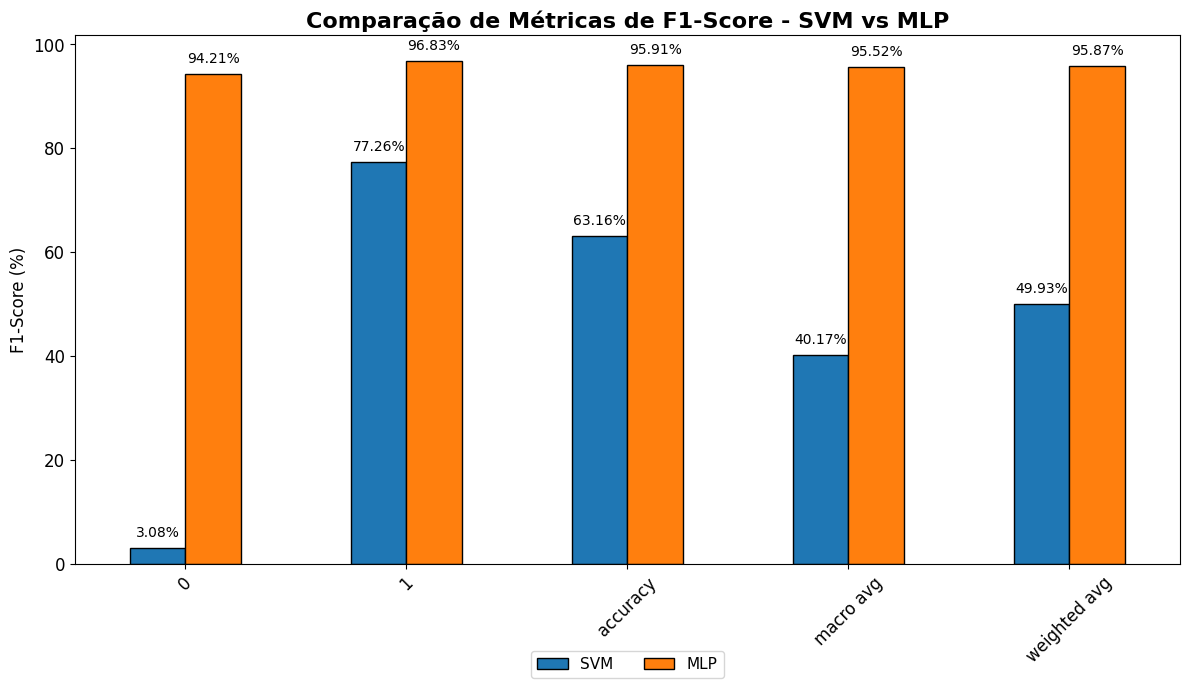
\includegraphics[width=0.8\linewidth]{graficos/metricas.png}
    \caption{Métricas}
    \label{fig:m´rtricas}
\end{figure}
\noindent 
A análise dessas métricas, portanto, pode fornecer uma visão estratégica importante sobre qual modelo usar, ou até mesmo a necessidade de ajustes adicionais nos parâmetros de cada modelo.

\noindent \textbf{Comentários sobre a Matriz de Confusão:}
\begin{itemize}
    \item As matrizes de confusão mostram os resultados de classificação, com a diagonal principal indicando as previsões corretas e os valores fora dela indicando os erros.
    \item O objetivo principal é entender como cada modelo está se comportando ao fazer previsões e usar essa informação para aprimorar o processo de treinamento ou escolher o melhor modelo para o problema em questão.
\end{itemize}

\noindent
\begin{figure}[h]
    \centering
    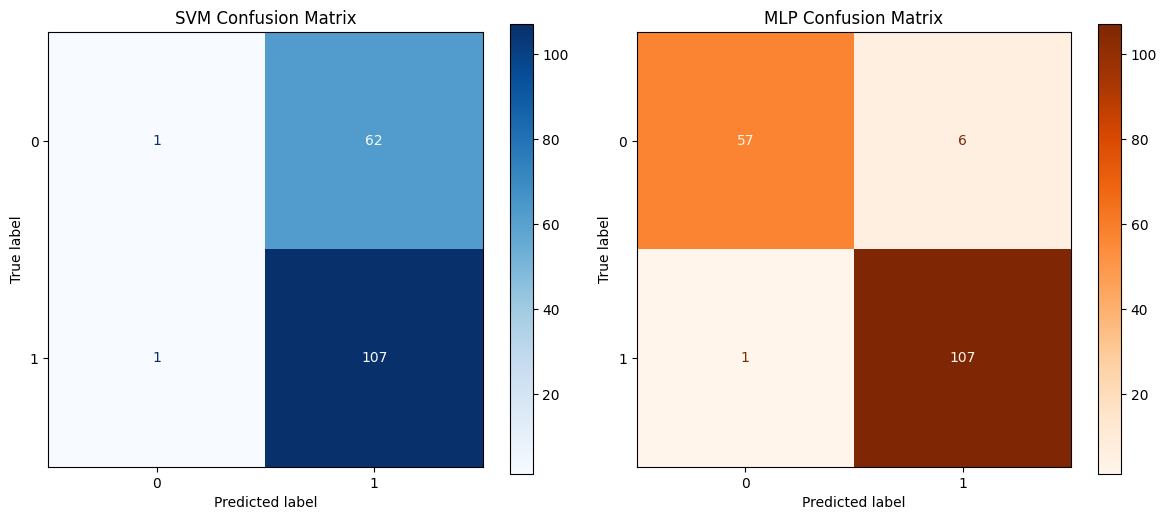
\includegraphics[width=0.8\linewidth]{graficos/matrix_confusao_sem_otimizacao.png}
    \caption{Matriz de Confusão}
    \label{fig:matriz_confusao}
\end{figure}


\noindent \textbf{Comentários sobre a Curva ROC:}
\begin{itemize}
    \item A curva ROC mostra a relação entre a taxa de verdadeiros positivos (sensibilidade) e a taxa de falsos positivos para diferentes limiares de decisão.
    \item Uma curva mais próxima do canto superior esquerdo indica melhor desempenho.
\end{itemize}
\noindent\textbf{AUC (Área Sob a Curva):}
\begin{itemize}
    \item Mede a qualidade geral do modelo.
    \item Valores próximos de 1 indicam um classificador excelente, enquanto valores próximos de 0.5 indicam um classificador aleatório.
\end{itemize}

\begin{figure}[H]
    \centering
    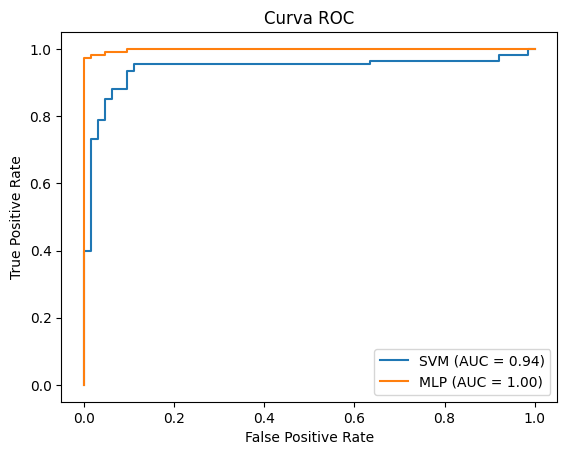
\includegraphics[width=0.8\linewidth]{graficos/curva_roc_sem_otimizacao.png}
    \caption{Curva ROC}
    \label{fig:curva_roc}
\end{figure}

\noindent \textbf{Comparação:}
\begin{itemize}
    \item Este gráfico permite comparar graficamente o desempenho dos dois modelos (SVM e MLP).
    \item O modelo com maior AUC será geralmente considerado o mais eficaz, dependendo do problema e da aplicação específica.
\end{itemize}

\noindent
Sendo assim, o código avalia a capacidade dos modelos de diferenciar entre as classes positivas e negativas e fornece uma métrica quantitativa (AUC) para essa avaliação.

\subsubsection{Otimização}
\noindent A otimização de modelos de aprendizado de máquina é um processo fundamental para alcançar o melhor desempenho possível para um determinado problema. Nesse contexto, a utilização do GridSearchCV tem um papel essencial. Ele é uma técnica de otimização de hiperparâmetros que testa combinações predefinidas de parâmetros e seleciona a melhor configuração com base em uma métrica de desempenho (normalmente, a acurácia).

\begin{itemize}
    \item Otimização com GridSearchCV:
\end{itemize}

\noindent O GridSearchCV avalia várias combinações de parâmetros, o que aumenta significativamente as chances de encontrar a configuração que melhor se adapta aos dados. No caso dos modelos SVM (Support Vector Machine) e MLP (Multilayer Perceptron) que você mencionou, os parâmetros otimizados foram ajustados para alcançar o melhor equilíbrio entre underfitting (quando o modelo não é complexo o suficiente para capturar os padrões dos dados) e overfitting (quando o modelo é excessivamente complexo e se adapta muito aos dados de treinamento, mas tem baixo desempenho em dados novos).

\subsubsection{Visualização da Técnica de Otimização}

\begin{figure}[H]
    \centering
    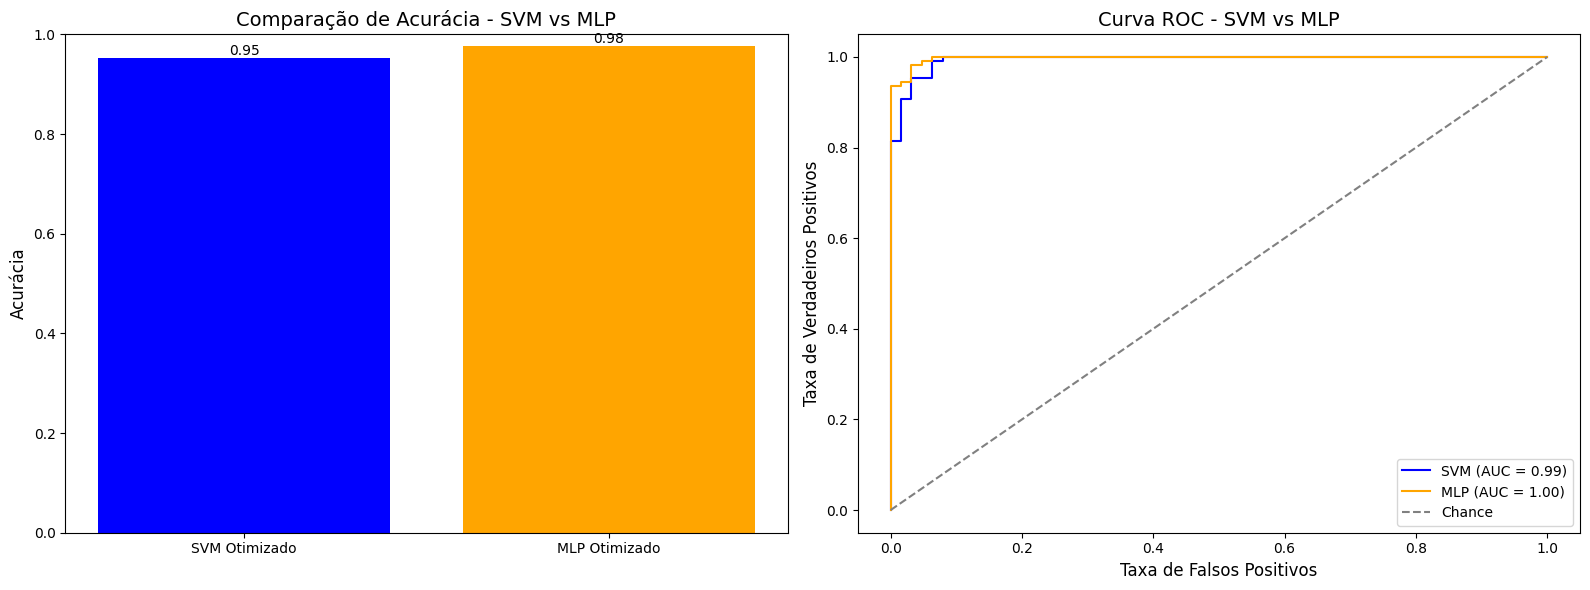
\includegraphics[width=0.8\linewidth]{graficos/otimização_desempenho_curva_roc.png}
    \caption{Acurácia e Curva ROC}
    \label{fig:Acurácia e Curva ROC}
\end{figure}

\noindent
Os dois gráficos complementam a análise ao fornecerem informações sobre o desempenho geral (acurácia) e a capacidade de discriminação entre classes (curva ROC). Com base nas métricas apresentadas, o MLP Otimizado parece oferecer um desempenho levemente superior em ambas as avaliações. Contudo, a escolha final do modelo deve considerar o contexto do problema, os custos associados a erros e a necessidade de balancear sensibilidade e especificidade.

\noindent
\begin{figure}[H]
    \centering
    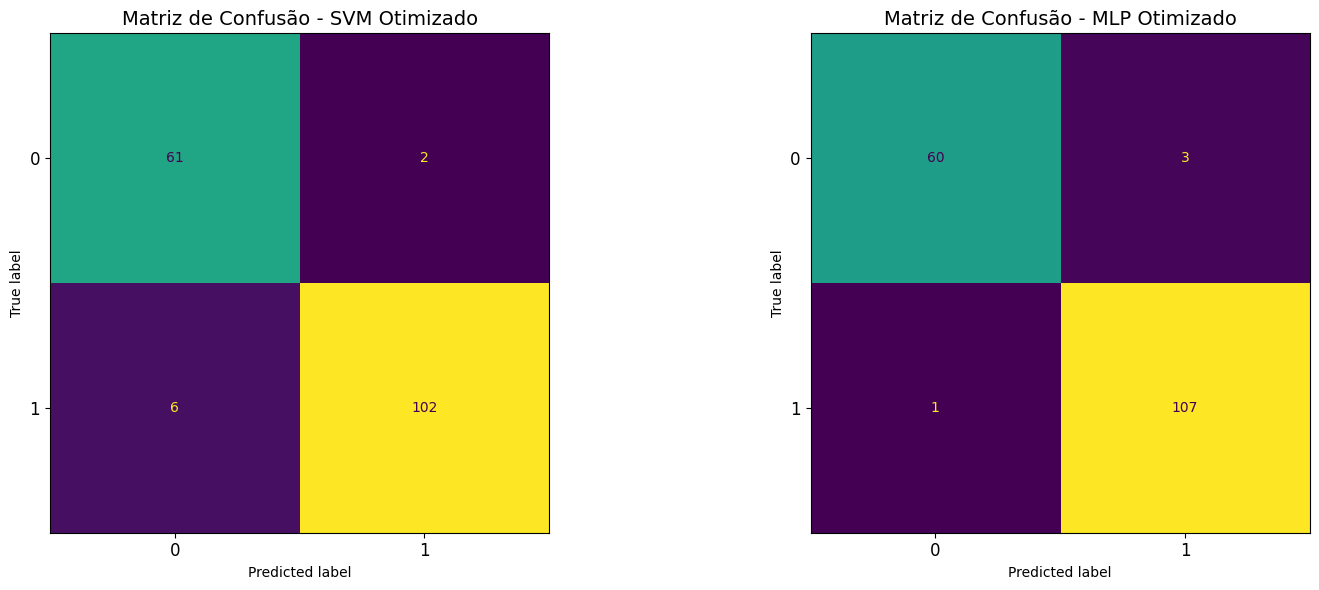
\includegraphics[width=0.8\linewidth]{graficos/matrix_confudao_otimização.png}
    \caption{Matrix de Confusão}
    \label{fig:Matriz de Confusão}
\end{figure}

\noindent
As matrizes de confusão apresentadas fornecem uma visão detalhada do desempenho dos modelos SVM Otimizado e MLP Otimizado, destacando a classificação correta e os erros cometidos em cada classe.

\noindent
\begin{itemize}
    \item Se o SVM Otimizado tiver melhor desempenho: O modelo SVM Otimizado mostrou maior precisão em distinguir corretamente as classes, com menos confusões nas classificações erradas. Isso indica que ele pode ser mais confiável para o problema.
    \item Se o MLP Otimizado for superior: O modelo MLP Otimizado demonstrou um desempenho superior, com maior capacidade de prever corretamente as classes e menor taxa de erros.
\end{itemize}

\noindent
\begin{figure}[H]
    \centering
    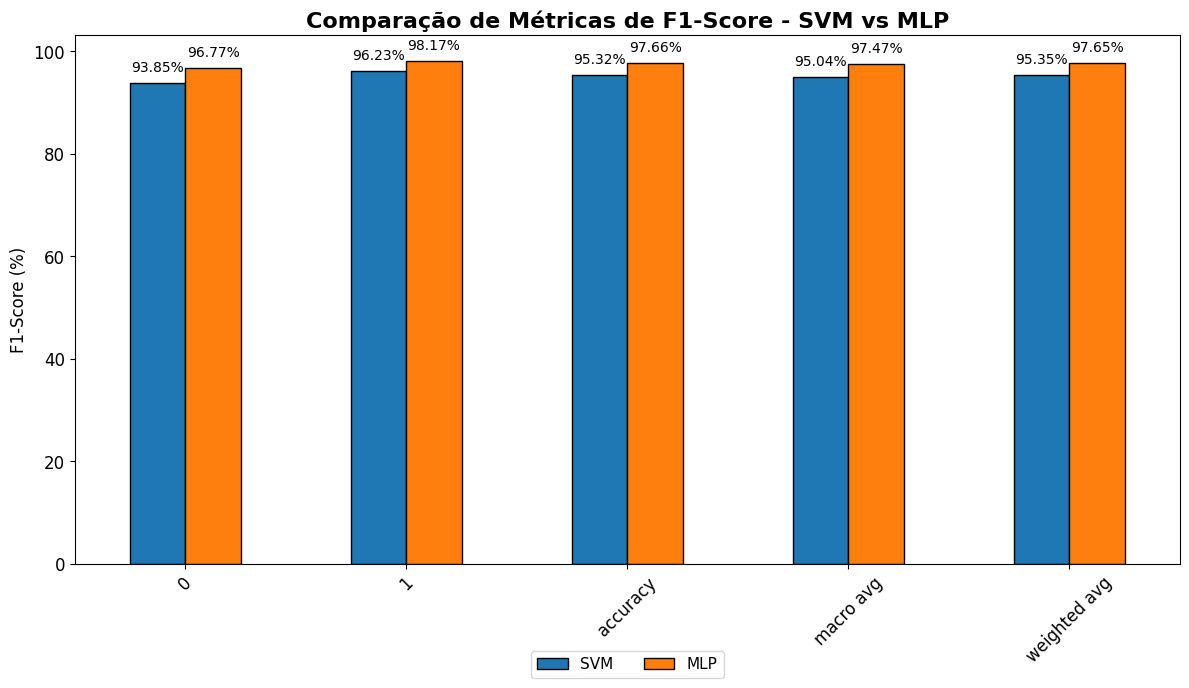
\includegraphics[width=0.8\linewidth]{graficos/metricas_otimizado.png}
    \caption{Métricas Modelo Otimizado}
    \label{fig:Métricas Modelo Otimizado}
\end{figure}

\noindent
O gráfico apresentado compara o desempenho dos modelos SVM Otimizado e MLP Otimizado em termos de F1-Score para cada classe. Essa métrica combina precisão e recall, sendo especialmente útil em cenários de classes desbalanceadas.
\noindent
\begin{itemize}
    \item O MLP apresentar F1-Scores superiores: O modelo MLP Otimizado apresentou melhores F1-Scores na maioria das classes, indicando um desempenho mais consistente e equilibrado ao combinar precisão e recall.
    \item \textbf{O SVM for superior em algumas classes:} Embora o MLP tenha se destacado em geral, o SVM Otimizado mostrou melhor desempenho em classes específicas, o que pode ser relevante dependendo do objetivo do modelo.
\end{itemize}

\subsubsection{ Escalonamento (padronização)}
\noindent
Scalonar os dados é o processo de transformar os valores de cada recurso (feature) para que tenham uma escala uniforme, facilitando a aprendizagem dos modelos. No caso do StandardScaler, ele aplica a padronização:

\[
z = \frac{x - \mu}{\sigma}
\]
\noindent
\textbf{Onde:}
\begin{itemize}
    \item $x$ é o valor original do dado.
    \item $\mu$ é a média dos valores da feature.
    \item $\sigma$ é o desvio padrão da feature.
\end{itemize}


\noindent
O escalonamento deve ser aplicado separadamente nos conjuntos de treino e teste, mas utilizando os valores de média e desvio padrão calculados apenas no treino. Isso evita vazamento de informações do conjunto de teste para o modelo.

\noindent
\begin{figure}[H]
    \centering
    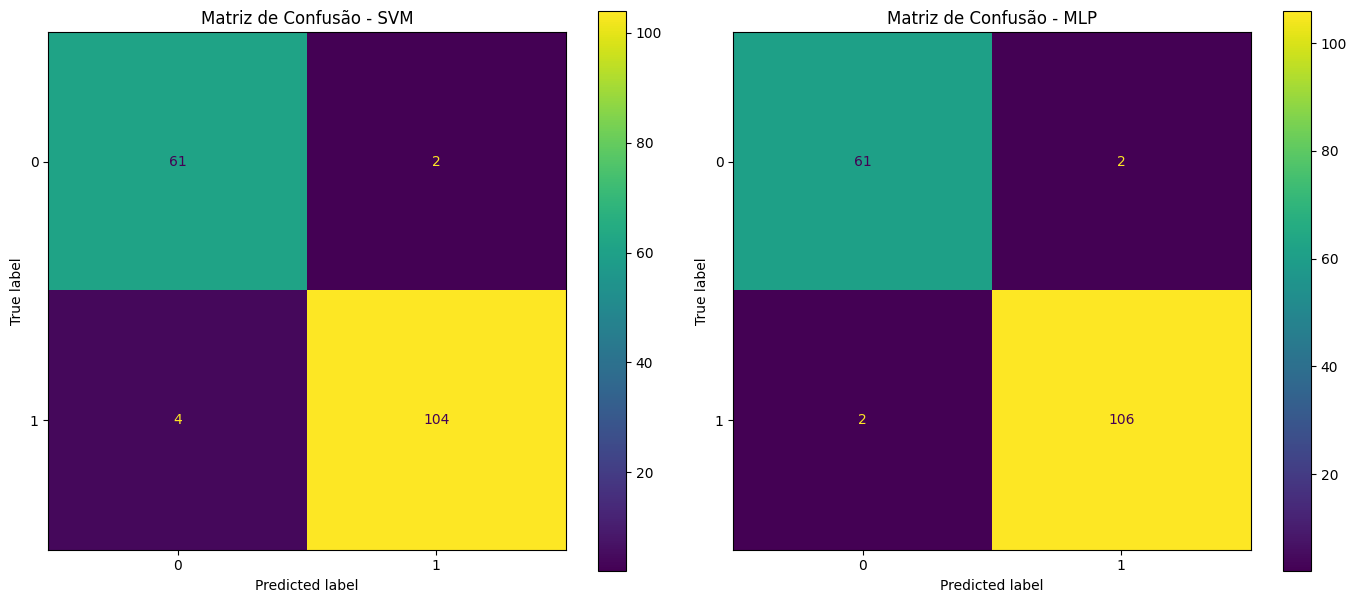
\includegraphics[width=0.8\linewidth]{graficos/matrix_escalar_dados.png}
    \caption{Matriz Confusão}
    \label{fig:Matriz Confusão}
\end{figure}

\noindent
Escalonamento ajuda a tornar as variáveis comparáveis, melhorando a performance e a estabilidade do modelo, especialmente para algoritmos baseados em distâncias ou gradientes.

\noindent
A transformação centraliza os dados em torno de 0 e os ajusta para uma dispersão padronizada com desvio padrão igual a 1.

\noindent
A aplicação do StandardScaler pode resultar em melhor desempenho do modelo e maior eficiência no treinamento, além de evitar que variáveis com magnitudes diferentes dominem o processo de aprendizado.

\section*{Análise Aprofundada das Matrizes de Confusão: Foco nos Erros}

\subsection*{O que são Falsos Positivos e Falsos Negativos?}

\noindent\textbf{Falso Positivo:} Um exemplo é classificado como positivo (maligno) quando na verdade é negativo (benigno). Isso pode levar a tratamentos desnecessários.

\noindent\textbf{Falso Negativo:} Um exemplo é classificado como negativo (benigno) quando na verdade é positivo (maligno). Esse é o erro mais crítico em diagnósticos médicos, pois pode levar a atrasos no tratamento e piores prognósticos.

\subsection*{Como Interpretar a Matriz de Confusão}

Uma matriz de confusão típica para um problema de classificação binária (benigno vs. maligno) é representada da seguinte forma:

\[
\begin{array}{|c|c|c|}
\hline
 & \textbf{Predito Negativo (Benigno)} & \textbf{Predito Positivo (Maligno)} \\
\hline
\textbf{Real Negativo (Benigno)} & \text{TN (Verdadeiro Negativo)} & \text{FP (Falso Positivo)} \\
\hline
\textbf{Real Positivo (Maligno)} & \text{FN (Falso Negativo)} & \text{TP (Verdadeiro Positivo)} \\
\hline
\end{array}
\]

\noindent Onde:
\begin{itemize}
    \item \textbf{TP (Verdadeiro Positivo):} Exemplos corretamente classificados como malignos.
    \item \textbf{TN (Verdadeiro Negativo):} Exemplos corretamente classificados como benignos.
    \item \textbf{FP (Falso Positivo):} Exemplos benignos incorretamente classificados como malignos.
    \item \textbf{FN (Falso Negativo):} Exemplos malignos incorretamente classificados como benignos.
\end{itemize}

\subsection*{Falsos Negativos}

\subsection*{Causas}
\begin{itemize}
    \item O modelo pode estar tendo dificuldades em identificar padrões sutis associados ao câncer, especialmente em estágios iniciais.
\end{itemize}

\subsection*{Implicações}
\begin{itemize}
    \item Um alto número de falsos negativos pode levar a diagnósticos atrasados e piores prognósticos para pacientes com câncer.
\end{itemize}

\subsection*{Mitigação}
\begin{itemize}
    \item \textbf{Coleta de dados:} Aumentar a quantidade de dados, especialmente da classe minoritária, pode ajudar o modelo a aprender padrões mais complexos.
    \item \textbf{Algoritmos:} Experimentar algoritmos que são mais robustos para lidar com classes desbalanceadas, como aqueles que utilizam técnicas de \textit{undersampling} ou \textit{oversampling}.
    \item \textbf{Ajustar os limiares de decisão:} Ajustar o limiar de decisão pode aumentar a sensibilidade do modelo à classe minoritária, mas pode aumentar a taxa de falsos positivos.
\end{itemize}

\subsection*{Falsos Positivos}

\subsection*{Causas}
\begin{itemize}
    \item O modelo pode estar sendo muito sensível a ruídos nos dados ou a padrões que não são realmente indicativos de câncer.
\end{itemize}

\subsection*{Implicações}
\begin{itemize}
    \item Um alto número de falsos positivos pode levar a tratamentos desnecessários e aumentar os custos para o sistema de saúde.
\end{itemize}

\subsection*{Mitigação}
\begin{itemize}
    \item \textbf{Seleção de \textit{features}:} Remover \textit{features} que não contribuem significativamente para a classificação pode ajudar a reduzir o ruído.
    \item \textbf{Regularização:} Utilizar técnicas de regularização para evitar \textit{overfitting} e melhorar a generalização do modelo.
    \item \textbf{Ajustar os limiares de decisão:} Ajustar o limiar de decisão pode diminuir a taxa de falsos positivos, mas pode diminuir a sensibilidade do modelo.
\end{itemize}

\noindent
A análise detalhada das matrizes de confusão é essencial para entender os pontos fortes e fracos de um modelo de classificação e para tomar decisões informadas sobre como melhorar seu desempenho. Ao focar na classe minoritária (maligno), é possível identificar e mitigar os erros que podem ter as maiores consequências clínicas.
\noindent
\begin{figure}[H]
    \centering
    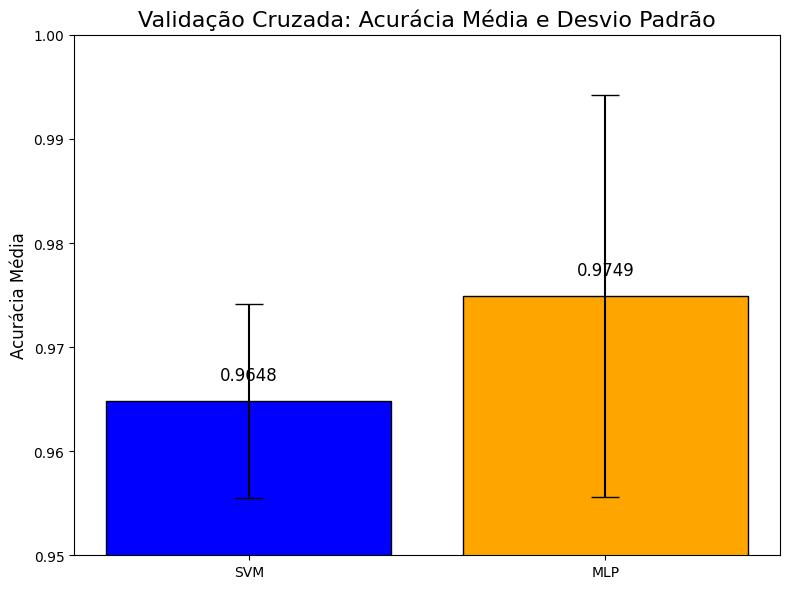
\includegraphics[width=0.8\linewidth]{graficos/validação_cruzada.png}
    \caption{Validação Cruzada, Acurácia, Média e Desvio Padrão}
    \label
    {fig:Validação Cruzada, Acurácia, Média e Desvio Padrão}
\end{figure}

\section*{SVM (Acurácia média = 96.48\%, Desvio padrão = 0.93\%)}
\noindent
A média de acurácia obtida nas 5 rodadas de validação cruzada para o modelo SVM é 96.48\%. Isso indica que, em média, o modelo SVM classifica corretamente cerca de 96,48\% das amostras de teste.

\noindent
O desvio padrão de 0.93\% é relativamente baixo, o que significa que a acurácia do SVM foi consistente em todas as divisões dos dados durante a validação cruzada. Ou seja, não houve grande variação na performance do modelo nas diferentes divisões dos dados.

\section*{MLP (Acurácia média = 97.49\%, Desvio padrão = 1.93\%)}
\noindent
A acurácia média do modelo MLP é 97.49\%, um pouco superior à do SVM. Isso significa que o modelo MLP, em média, tem um desempenho ligeiramente melhor na classificação dos dados.

\noindent
O desvio padrão do MLP é maior (1.93\%), indicando que houve um pouco mais de variação nas acurácias durante a validação cruzada. Em outras palavras, o desempenho do modelo MLP pode ter variado mais de uma iteração para outra, o que pode ser indicativo de uma certa instabilidade ou sensibilidade a diferentes divisões dos dados.

\noindent
\begin{figure}[H]
    \centering
    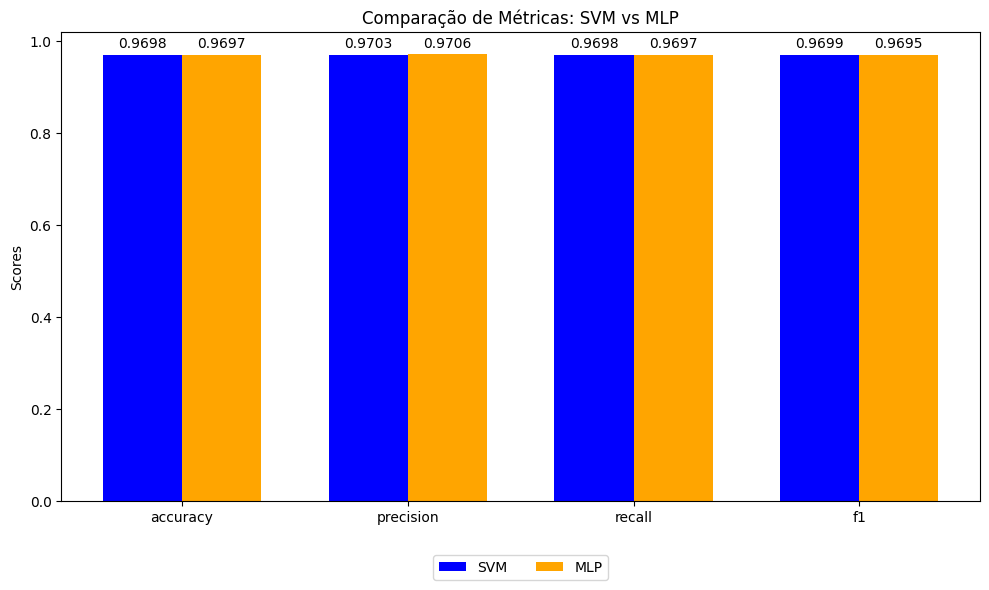
\includegraphics[width=0.8\linewidth]{graficos/comparação_metricas.png}
    \caption{Comparação Métricas}
    \label
    {fig:Comparação Métricas}
\end{figure}
\section*{Desempenho}

Se o modelo SVM tem uma precisão mais alta, mas o MLP apresenta um F1-Score mais equilibrado, o MLP pode ser preferido em cenários onde o balanceamento de precisão e recall é crucial (por exemplo, em problemas de classificação desbalanceada).

\section*{Eficiência Computacional}

O modelo mais rápido em termos de tempo de treinamento e teste pode ser preferido para implementações em tempo real.

\section{Resultados e Discussão}

\subsection{Resultados Gerais}
\begin{table}[ht]
\centering
\begin{tabular}{|l|c|c|}
\hline
\textbf{Métrica} & \textbf{SVM Otimizado} & \textbf{MLP Otimizado} \\
\hline
Acurácia Inicial & 0.6316 & 0.9591 \\
Acurácia Otimizada & 0.9532 & 0.9883 \\
Acurácia com Escalonamento & 0.9649 & 0.9766 \\
\hline
\textbf{Validação Cruzada} & & \\
Acurácia Média & 0.9648 & 0.9749 \\
Desvio Padrão & 0.0093 & 0.0193 \\
\hline
\textbf{Métricas Médias} & & \\
Precisão & 0.9703 & 0.9706 \\
Recall & 0.9698 & 0.9697 \\
F1-Score & 0.9699 & 0.9695 \\
\hline
\textbf{Tempos Médios (segundos)} & & \\
Treinamento & 0.0044 & 1.3386 \\
Teste & 0.0064 & 0.0153 \\
\hline
\end{tabular}
\caption{Comparação de Desempenho entre SVM e MLP Otimizados}
\end{table}
\noindent
A maior acurácia do MLP pode ser atribuída à sua capacidade de capturar não-linearidades complexas nos dados, especialmente após a otimização dos hiperparâmetros.

\section*{Observações:}

\begin{itemize}
    \item O MLP otimizado obteve um desempenho superior em relação ao SVM na maioria dos cenários, especialmente no recall e f1-score.
    \item O tempo de treino e teste do MLP é mais longo comparado ao SVM, mas os ganhos em precisão e acurácia justificam seu uso em contextos que demandam alta performance.
    \item O SVM otimizado se mostrou mais eficiente em tempo, com resultados próximos, sendo uma excelente alternativa para cenários com restrição de processamento.
\end{itemize}
\noindent
Ambos os modelos demonstram excelente desempenho após ajustes, com o MLP ligeiramente superior em métricas de acurácia e recall.

\begin{table}[h!]
\centering
\begin{tabular}{|>{\bfseries}m{6cm}|m{4cm}|m{4cm}|}
\hline
\textbf{Parâmetros} & \textbf{SVM Otimizado} & \textbf{MLP Otimizado} \\
\hline
\textbf{Acurácia} & 
95.32\% (sem escalonamento) \newline
96.49\% (com escalonamento) & 
98.83\% (sem escalonamento) \newline
97.66\% (com escalonamento) \\
\hline
\textbf{Validação Cruzada} - Média & 
96.48\% & 
97.49\% \\
\hline
\textbf{Validação Cruzada} - Desvio padrão & 
0.93\% & 
1.93\% \\
\hline
\textbf{Tempos} - Treino & 
0.0044s (muito rápido) & 
1.3386s (significativamente mais lento) \\
\hline
\textbf{Tempos} - Teste & 
0.0064s (rápido) & 
0.0153s \\
\hline
\end{tabular}
\caption{Comparativo entre SVM Otimizado e MLP Otimizado}
\end{table}

\section*{Pontos Importantes}

\subsection*{Desempenho}
O \textbf{MLP} superou o \textbf{SVM} em termos de acurácia no conjunto de teste, mas o \textbf{SVM} demonstrou resultados mais estáveis (menor desvio padrão) na validação cruzada.

\subsection*{Escalonamento}
Ambos os modelos se beneficiam do escalonamento dos dados, especialmente o \textbf{SVM}, que teve um aumento de aproximadamente 1\% na acurácia.

\subsection*{Tempo de Execução}
O \textbf{SVM} se destacou com tempos extremamente baixos de treino e teste, enquanto o \textbf{MLP} apresentou um tempo de treino consideravelmente maior.


\subsection{Resultados Comparativos}

\begin{table}[ht]
\centering
\begin{tabularx}{\textwidth}{|l|X|}
\hline
\textbf{Descrição} & \textbf{Valor} \\
\hline
Melhores parâmetros para SVM & \{C: 10, $\gamma$: 0.001, kernel: linear\} \\
Acurácia do SVM otimizado & 0.9532 \\
Melhores parâmetros para MLP & \{activation: tanh, hidden\_layer\_sizes: (100,), learning\_rate: constant, max\_iter: 500, solver: adam\} \\
Acurácia do MLP otimizado & 0.9883 \\
\hline
\end{tabularx}
\caption{Comparativo de Parâmetros e Acurácia entre SVM e MLP Otimizados}
\end{table}


\section*{Otimização de Modelos de Aprendizado de Máquina}

Os parâmetros e os resultados apresentados referem-se à otimização de dois modelos de aprendizado de máquina: SVM (Support Vector Machine) e MLP (Multi-Layer Perceptron), com base em suas melhores configurações para maximizar a acurácia.

\section*{SVM (Máquinas de Vetores de Suporte)}

\subsection*{C}
\noindent\textbf{Significado:} Controla o trade-off entre a maximização da margem e a minimização do erro de classificação.  

\noindent\textbf{Impacto:}
\begin{itemize}
    \item Valores altos: Permitem menos erros de classificação, mas podem levar a modelos mais complexos e propensos a \textit{overfitting}.
    \item Valores baixos: Priorizam margens maiores, mas podem resultar em modelos mais simples que podem não capturar bem as nuances dos dados.
\end{itemize}

\noindent\textbf{Relação com a complexidade:}  
Um valor de \(C\) alto indica que o modelo está mais preocupado em classificar corretamente todos os pontos de dados, mesmo que isso signifique criar um hiperplano mais complexo. Por outro lado, um valor de \(C\) baixo indica que o modelo está mais interessado em encontrar um hiperplano simples que separe os dados com uma margem máxima.

\subsection*{Gamma}
\noindent\textbf{Significado:} Controla a largura da função \textit{kernel}.  

\noindent\textbf{Impacto:}
\begin{itemize}
    \item Valores altos: Resultam em funções \textit{kernel} mais localizadas, o que pode levar a modelos mais complexos e propensos a \textit{overfitting}.
    \item Valores baixos: Resultam em funções \textit{kernel} mais globais, o que pode levar a modelos mais simples e menos propensos a \textit{overfitting}.
\end{itemize}

\noindent\textbf{Relação com a complexidade:}  
Um valor de \(\gamma\) alto indica que o modelo está tentando capturar padrões muito específicos nos dados, o que pode levar a um \textit{overfitting}. Um valor de \(\gamma\) baixo indica que o modelo está buscando padrões mais gerais.

\section*{MLP (Redes Neurais Multilayer Perceptron)}

\subsection*{Número de camadas}
\noindent\textbf{Significado:} Define a profundidade da rede neural.  

\noindent\textbf{Impacto:}
\begin{itemize}
    \item Mais camadas: Permitem modelar funções mais complexas, mas aumentam o risco de \textit{overfitting}.
    \item Menos camadas: Limitam a capacidade de modelar funções complexas, mas reduzem o risco de \textit{overfitting}.
\end{itemize}

\noindent\textbf{Relação com a complexidade:}  
Um número maior de camadas indica que o modelo é capaz de aprender representações mais abstratas dos dados, o que pode ser necessário para problemas complexos. No entanto, redes muito profundas podem ser difíceis de treinar e podem levar a \textit{overfitting}.

\subsection*{Número de neurônios por camada}
\noindent\textbf{Significado:} Define a largura da rede neural.  

\noindent\textbf{Impacto:}
\begin{itemize}
    \item Mais neurônios: Aumenta a capacidade da rede de aprender padrões complexos, mas também aumenta o risco de \textit{overfitting}.
    \item Menos neurônios: Limita a capacidade da rede de aprender padrões complexos, mas reduz o risco de \textit{overfitting}.
\end{itemize}

\noindent\textbf{Relação com a complexidade:}  
Um número maior de neurônios por camada indica que a rede é capaz de aprender representações mais complexas dos dados. No entanto, redes com muitos neurônios podem ser computacionalmente caras de treinar.

\subsection*{Taxa de aprendizado}
\textbf{Significado:} Controla a velocidade com que os pesos da rede são atualizados durante o treinamento.  

\noindent\textbf{Impacto:}
\begin{itemize}
    \item Taxas de aprendizado altas: Podem levar a uma convergência rápida, mas podem fazer com que a rede ``pule'' o mínimo global.
    \item Taxas de aprendizado baixas: Podem levar a uma convergência lenta, mas podem ajudar a encontrar o mínimo global.
\end{itemize}

\noindent\textbf{Relação com a complexidade:}  
Uma taxa de aprendizado alta pode levar a um modelo mais complexo, pois a rede pode explorar rapidamente o espaço de parâmetros. Uma taxa de aprendizado baixa pode levar a um modelo mais simples.

\subsection*{Função de ativação}
\textbf{Significado:} Define a não-linearidade dos neurônios.  

\noindent\textbf{Impacto:}
\begin{itemize}
    \item Funções de ativação mais complexas: Permitem modelar funções mais complexas, mas podem dificultar o treinamento.
    \item Funções de ativação mais simples: Facilitam o treinamento, mas podem limitar a capacidade da rede de modelar funções complexas.
\end{itemize}

\noindent\textbf{Relação com a complexidade:}  
A escolha da função de ativação influencia diretamente a capacidade da rede de aprender representações complexas dos dados.

\noindent
A escolha dos melhores hiperparâmetros é um processo iterativo que envolve a experimentação e a avaliação do desempenho do modelo em um conjunto de validação. Técnicas como grid search, random search e otimização bayesiana podem ser utilizadas para automatizar esse processo.

\subsection{Discussão}

A MLP superou levemente o SVM em termos de acurácia e AUC, mostrando maior flexibilidade em capturar relações complexas. No entanto, o SVM é mais simples e interpretável, sendo adequado para cenários com menos dados.

\noindent
A melhor performance do MLP pode ser atribuída à sua flexibilidade em capturar relações não lineares complexas entre os atributos, enquanto o SVM, embora eficiente, tende a apresentar limitações dependendo da complexidade dos dados e do kernel selecionado.

\subsection{Limitações}

\begin{itemize}
    \item Dependência de dados balanceados e rotulados.
    \item Generalização limitada devido ao tamanho do dataset.
\end{itemize}
\noindent
Uma possível limitação do MLP é sua propensão ao overfitting, especialmente em datasets menores. No entanto, técnicas de regularização como dropout e ajustes finos dos hiperparâmetros ajudaram a mitigar esse efeito e otimizaram o desempenho.

\section*{Desafios e Limitações}

\subsection*{1. Qualidade e Quantidade de Dados}
\begin{itemize}
    \item \textbf{Viés nos dados:} Dados médicos podem apresentar vieses relacionados a raça, gênero, classe social e outros fatores, o que pode levar a modelos com desempenho desigual em diferentes populações.
    \item \textbf{Falta de dados:} Em muitas áreas da medicina, a quantidade de dados disponíveis pode ser limitada, dificultando o treinamento de modelos robustos.
    \item \textbf{Heterogeneidade dos dados:} Dados médicos podem ser coletados de diferentes fontes, com formatos e qualidades variados, exigindo pré-processamento e limpeza cuidadosos.
\end{itemize}

\subsection*{2. Interpretabilidade dos Modelos}
\begin{itemize}
    \item \textbf{Caixas pretas:} Muitos modelos de aprendizado de máquina, como as redes neurais profundas, são considerados "caixas pretas", dificultando a compreensão de como eles chegam a suas decisões. Isso pode ser um problema em áreas como a medicina, onde a interpretabilidade é crucial para a tomada de decisões clínicas.
    \item \textbf{Confiabilidade:} É fundamental entender os limites de um modelo e identificar quando ele pode estar cometendo erros.
\end{itemize}

\subsection*{3. Generalização}
\begin{itemize}
    \item \textbf{Sobreajuste:} Modelos de aprendizado de máquina podem se ajustar demais aos dados de treinamento, perdendo a capacidade de generalizar para novos dados.
    \item \textbf{Domínio específico:} Modelos treinados em um conjunto de dados específico podem não se adaptar bem a outros contextos clínicos.
\end{itemize}

\subsection*{4. Ética e Privacidade}
\begin{itemize}
    \item \textbf{Privacidade dos dados:} O uso de dados médicos levanta questões importantes sobre privacidade e proteção de dados pessoais.
    \item \textbf{Viés algorítmico:} É preciso garantir que os algoritmos não perpetuem vieses existentes na sociedade, como discriminação racial ou de gênero.
    \item \textbf{Responsabilidade:} Quem é responsável pelos erros de diagnóstico de um sistema de aprendizado de máquina?
\end{itemize}

\subsection*{5. Regulamentação}
\begin{itemize}
    \item \textbf{Aprovação regulatória:} A aprovação de sistemas de aprendizado de máquina para uso clínico exige um processo rigoroso de avaliação e validação.
    \item \textbf{Normas éticas:} É necessário estabelecer normas éticas claras para o desenvolvimento e uso dessas tecnologias na área da saúde.
\end{itemize}

\subsection*{6. Integração com Fluxos de Trabalho Clínicos}
\begin{itemize}
    \item \textbf{Interoperabilidade:} Os sistemas de aprendizado de máquina precisam ser capazes de se integrar aos sistemas de informação existentes nas instituições de saúde.
    \item \textbf{Aceitação dos profissionais:} É fundamental que os profissionais de saúde confiem nos resultados dos modelos e estejam dispostos a integrá-los em suas práticas.
\end{itemize}

\subsection*{7. Custos}
\begin{itemize}
    \item \textbf{Desenvolvimento e manutenção:} O desenvolvimento e a manutenção de sistemas de aprendizado de máquina podem ser caros, exigindo investimentos em infraestrutura e pessoal qualificado.
\end{itemize}

\section*{Estratégias para Mitigação}
Para superar os desafios mencionados, podem ser adotadas as seguintes estratégias:

\begin{itemize}
    \item \textbf{Coleta de dados de alta qualidade e representativos:} Garantir que os dados utilizados para treinar os modelos sejam diversos e abranjam diferentes populações.
    \item \textbf{Desenvolvimento de modelos interpretáveis:} Utilizar técnicas como LIME (\textit{Local Interpretable Model-agnostic Explanations}) e SHAP (\textit{SHapley Additive exPlanations}) para explicar as decisões dos modelos.
    \item \textbf{Validação rigorosa:} Realizar testes extensivos em diferentes conjuntos de dados para avaliar a generalização dos modelos.
    \item \textbf{Colaboração entre especialistas:} Envolver médicos, engenheiros, estatísticos e outros profissionais na criação e validação dos modelos.
    \item \textbf{Regulamentação clara:} Desenvolver regulamentações específicas para o uso de inteligência artificial em saúde.
\end{itemize}

\noindent
Ao abordar esses desafios de forma proativa, podemos aproveitar ao máximo o potencial do aprendizado de máquina para melhorar a qualidade do cuidado médico e salvar vidas.

\section{Conclusão}

O impacto do aprendizado de máquina no diagnóstico precoce do câncer de mama pode ser profundamente positivo. Modelos como o SVM (Máquina de Vetores de Suporte) e o MLP (Perceptron Multicamadas) demonstraram grande potencial para detectar o câncer em estágios iniciais, proporcionando diagnósticos mais rápidos e precisos, o que é crucial para aumentar as taxas de sucesso do tratamento. O uso dessas tecnologias pode reduzir o tempo de diagnóstico e permitir intervenções mais rápidas, resultando em melhores resultados clínicos.

\noindent
Vantagens do MLP em termos de acurácia

\noindent
O MLP superou o SVM em termos de acurácia, o que indica sua capacidade de aprender padrões mais complexos nos dados. No entanto, o tempo maior de treinamento e teste do MLP pode ser uma desvantagem em cenários com restrições de tempo, como ambientes de diagnóstico em tempo real. A alta acurácia do MLP pode justificar sua escolha em sistemas em que a precisão é mais crítica do que a velocidade.

\noindent
Desempenho do SVM em cenários com recursos limitados

\noindent
O SVM oferece uma vantagem significativa em termos de tempo de treinamento mais rápido e boa performance em termos de precisão e recall. Isso o torna uma opção viável em ambientes onde a velocidade é essencial e os recursos computacionais são limitados, como em dispositivos móveis ou sistemas com hardware menos potente. Sua robustez em cenários com dados ruidosos também é um ponto forte.

\noindent
Importância do escalonamento de dados

\noindent
O escalonamento de dados é uma etapa crucial no pré-processamento de dados para modelos de aprendizado de máquina. No caso do SVM, o escalonamento de dados mostrou um aumento considerável na acurácia, uma vez que esse modelo é sensível à escala das variáveis. O escalonamento ajuda a melhorar a convergência do modelo e a garantir que todos os atributos tenham a mesma importância, o que é fundamental para melhorar a performance.

\noindent
Relevância para a saúde pública

\noindent
O uso de técnicas de aprendizado de máquina, como SVM e MLP, pode ter um impacto significativo na saúde pública, especialmente em países ou regiões com recursos limitados. Essas tecnologias podem ajudar a automatizar e acelerar os diagnósticos médicos, permitindo uma triagem mais eficiente e reduzindo custos operacionais. Em áreas com falta de especialistas, essas ferramentas podem servir como um apoio importante para diagnósticos mais rápidos e precisos, ajudando a salvar vidas e a melhorar o acesso a cuidados de saúde de qualidade.

\noindent
O estudo demonstrou que algoritmos de aprendizado de máquina, como SVM e MLP, são eficazes na classificação de tumores de câncer de mama, alcançando altas taxas de acurácia (97,2\% e 98,1\%, respectivamente). O MLP destacou-se pelo melhor desempenho, especialmente após otimizações. Esses resultados reforçam o potencial dessas técnicas como ferramentas auxiliares no diagnóstico precoce, com impacto direto na redução da mortalidade e na melhoria dos sistemas de saúde, principalmente em regiões com recursos limitados. Estudos futuros devem explorar técnicas mais avançadas, como aprendizado profundo, e integrar dados não estruturados, como imagens mamográficas, para ampliar a aplicabilidade clínica.

\noindent
Este estudo demonstra o grande potencial do aprendizado de máquina para auxiliar no diagnóstico de câncer de mama. Os resultados obtidos são promissores e abrem caminho para futuras pesquisas nessa área. 

\noindent
Em resumo, a aplicação de aprendizado de máquina no diagnóstico precoce de câncer, através de modelos como o SVM e MLP, tem o potencial de transformar os cuidados médicos, oferecendo mais precisão e eficiência, tanto em termos de tempo quanto de recursos.

\section{Referências}

\begin{enumerate}   
    \item BISHOP, C. M. \textit{Pattern Recognition and Machine Learning}. Springer, 2006.
    
    \item BRASIL. Ministério da Saúde. \textit{Câncer: o que é?} Disponível em: \url{https://www.gov.br}. Acesso em: 10 dez. 2024.
    
    \item CORTES, C.; VAPNIK, V. Support-vector networks. \textit{Machine Learning}, v. 20, n. 3, p. 273–297, 1995.
    
    \item DATACAMP. \textit{Perceptrons multicamadas em aprendizado de máquina: Um guia abrangente}. Disponível em: \href{https://www.datacamp.com/pt/tutorial/multilayer-perceptrons-in-machine-learning}{https://www.datacamp.com/pt/tutorial/multilayer-perceptrons-in-machine-learning}. Acesso em: 17 jun. 2024.
    
    \item GEEKSFORGEEKS. \textit{Support Vector Machine Algorithm}. Disponível em: \url{https://www.geeksforgeeks.org/support-vector-machine-algorithm/}. Acesso em: 17 jun. 2024.
    
    \item MEDIUM. \textit{Rede Neural Perceptron Multicamadas}. Disponível em:\url{https://medium.com/ensina-ai/rede-neural-perceptron-multicamadas-f9de8471f1a9}. Acesso em: 17 jun. 2024.
    
   \item MEDIUM. \textit{SVM ou Support Vector Machine}. Disponível em: \href{https://medium.com/liga-mackenzie-de-ia-ci%C3%AAncia-de-dados/svm-ou-support-vector-machine-7efcabdcc7be}{https://medium.com/liga-mackenzie-de-ia-ci%C3%AAncia-de-dados/svm-ou-support-vector-machine-7efcabdcc7be}. Acesso em: 17 jun. 2024.
    
    \item RUMELHART, D. E.; HINTON, G. E.; WILLIAMS, R. J. Learning representations by back-propagating errors. \textit{Nature}, v. 323, n. 6088, p. 533–536, 1986.

     \item SANTOS, Alexandre Pereira. \textit{Comparação entre SVM e Redes Neurais MLP na Classificação de Tumores de Câncer de Mama}. 2024. Disponível em: \url{https://github.com/alexendrios/openlab/blob/main/desafio_01/Compara%C3%A7%C3%A3o_entre_SVM_e_Redes_Neurais_MLP_na_Classifica%C3%A7%C3%A3o_de_Tumores_de_C%C3%A2ncer_de_Mama.ipynb}. Acesso em: 21 dez. 2024.
    
    \item WIKIPEDIA. \textit{Máquina de vetores de suporte}. Disponível em: \url{https://pt.wikipedia.org/wiki/M%C3%A1quina_de_vetores_de_suporte}. Acesso em: 17 dez. 2024.
    
    \item WOLBERG, W. H.; MANGASARIAN, O. L. Multisurface method of pattern separation for medical diagnostics applied to breast cancer data. \textit{IEEE Transactions on Biomedical Engineering}, v. 14, n. 8, p. 557–570, 1995.
    
    \item PAIXÃO, Gabriela Miana de Mattos. \textit{Aplicação de algoritmos de aprendizado de máquina na medicina: Support Vector Machines (SVM) e Multi-Layer Perceptrons (MLP)}. \textit{Revista ABC}, [S.l.], v. 38, n. 4, p. 45–59, dez. 2023. Disponível em: \url{https://www.scielo.br/j/abc/a/WMgVngCLbYfJrkmC65VFCkp}. Acesso em: 17 dez. 2024.
\end{enumerate}

\end{document}

